\section{Related Work} \label{sec:related_work}
% \ha{long-tailed}
\subsection{Problem Setup}
We begin by reviewing the problem formulation for imbalanced multi-class classification. We consider the imbalanced $K$-class classification problem, where $K > 2$. Given a training dataset $\mathcal{D} = \{(\mathbf{x}_1, y_1), \dots, (\mathbf{x}_n, y_n)\}$, each input $\mathbf{x}_i \in \mathcal{X} \subseteq \mathbb{R}^d$ represents a feature vector, and its corresponding label $y_i \in \mathcal{Y} \subseteq \mathbb{R}^K$ is drawn from the joint distribution $P_{\mathbf{x}, y}^{\text{all}}$. The objective is to learn a classifier $f_{\mathbf{x}} \colon \mathbb{R}^d \to \mathbb{R}^K$ that minimizes the standard loss function:  
$L(\theta) = \mathbb{E}_{\mathbf{x}, y \sim P_{\mathbf{x}, y}^{\text{all}}} [\ell(f(\mathbf{x}), y)],$
where $\ell(\cdot, \cdot)$ is a predefined loss function, and $e_y$ denotes the one-hot encoded vector corresponding to label $y$. The predicted label $\hat{y}$ for an instance $\mathbf{x}$ is determined using the argmax function:  
$\hat{y} = \mathop{\arg\max}_{k \in K} f(\mathbf{x})_k,$
where $f(\mathbf{x})_k$ is the $k^{\text{th}}$ component of the output of $f(\mathbf{x})$.  
Let $n_j$ denote the size of class $j$. We assume the training dataset is \textit{imbalanced}, meaning the size of the largest class, $\max_i n_i$, differs significantly from that of the smallest class, $\min_i n_i$. The \textit{class imbalance ratio}, $\rho$, quantifies the degree of imbalance and is defined as:  
$\rho = \max_i n_i / \min_i n_i.$
This ratio serves as a measure of the imbalance of the dataset, with larger $\rho$ values indicating greater imbalance. In this context, the larger classes are referred to as the \emph{majority}, while the smaller ones are termed the \emph{minority}.  
After training $f(\mathbf{x})$ on the \textit{imbalanced} dataset, we follow the evaluation procedure outlined in~\cite{cao2019learning, cheng2023smote}. Specifically, the classifier is tested on a \textit{balanced} test set generated from the same conditional distribution $P(\mathbf{x} \mid y)$ for each class. This evaluation approach ensures equal importance is given to each class during testing, providing a fair assessment of the classifier's performance across all classes.
%%%% HA comment 22 Oct, 2025
% \textbf{Hybrid approaches} combine data-level and algorithm-level strategies to leverage the strengths of both and achieve more robust performance. These methods often integrate resampling techniques directly into the training process of an algorithm. For example, a popular hybrid strategy involves combining sampling methods with ensemble learning, such as creating balanced data subsets for each learner in a bagging or boosting framework.

\subsection{Imbalanced Learning Approaches}
\label{Mixup_interpolation}
To address the challenges, traditional solutions are broadly categorized into two families: \textit{data-oriented approaches} and \textit{algorithm-oriented approaches}.

% \textbf{Data-oriented approaches} directly address class imbalance by manipulating the training dataset itself to create a more balanced distribution. This is typically achieved by either oversampling the minority class to increase its representation or undersampling the majority class to reduce its dominance. Techniques range from simple random replication to more sophisticated synthetic sample generation methods like the SMOTE \cite{chawla2002smote}, which creates new minority instances by interpolating between existing ones.

% \textbf{Algorithm-oriented approaches}, in contrast, modify the learning algorithm to be more sensitive to the minority class without altering the training data. The most common strategy is cost-sensitive learning, which adjusts the model's objective function to assign higher misclassification penalties to errors made on minority class instances. This forces the model to prioritize learning the characteristics of underrepresented classes, effectively shifting the decision boundary to improve their recognition.

\paragraph{Data-oriented approaches} At the data level, methods reshape the training distribution to alleviate imbalance prior to optimization. While SMOTE \cite{chawla2002smote} remains a cornerstone, many extensions improve sample quality and coverage. For instance, k-Means SMOTE \cite{douzas2018improving} synthesizes minority examples within cluster-consistent regions, and reinforcement learning–based resampling \cite{fan2021imbalanced} adaptively selects/weights samples to maximize downstream accuracy. Beyond pure resampling, data augmentation has proven especially effective. Mixup \cite{zhang2017Mixup} constructs virtual examples by linearly interpolating pairs of inputs and labels, encouraging smoother decision boundaries and reducing overfitting to majority classes. These examples are generated via simple linear combinations as follows:

\begin{equation}
\label{mixup_x}
\tilde{\mathbf{x}} = \lambda \mathbf{x}_i + (1 - \lambda) \mathbf{x}_j,
\end{equation}
\begin{equation}
\label{mixup_y}
\tilde{y} = \lambda y_i + (1 - \lambda) y_j,
\end{equation}
where: \( (\mathbf{x}_i, y_i) \) and \( (\mathbf{x}_j, y_j) \) are two examples drawn from the training data using a sampling strategy (e.g., uniform, class-weighted, or oversampling). $\lambda \sim \mathit{Beta}(\gamma, \gamma)$ distribution.
\begin{figure}[htb]
    \centering
        \centering
        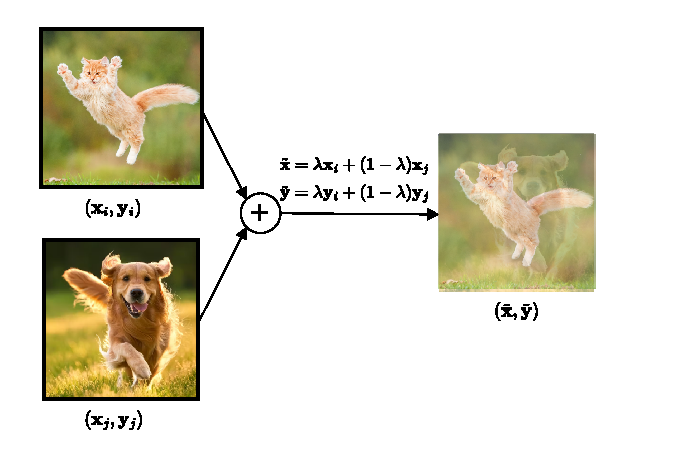
\includegraphics[width=0.9\columnwidth]{imbalanced.pdf}
        \caption{Illustration of the Mixup data augmentation technique. Two training samples 
     $(x_i, y_i)$ and $(x_j, y_j)$ are linearly combined with a mixing coefficient 
    $\lambda_x \sim \mathit{Beta}(\gamma, \gamma)$\ to generate a new virtual sample $(\tilde{x}, \tilde{y})$.}
\label{fig:cifar10_imbalance_mixup}
\end{figure}

By incorporating different sampling methods, such as class-weighted or oversampling, the technique ensures that underrepresented classes are more frequently sampled, mitigating the impact of class imbalance. Sampling-based Mixup has been shown to enhance the diversity of training data, reduce the memorization of corrupt labels, improve robustness to adversarial training, and boost the generalizability of deep networks. This approach is particularly beneficial for tasks with severe class imbalance, leading to improved performance across a variety of image classification tasks.

\paragraph{Algorithm-Oriented Approaches} Algorithm-level strategies modify the learning objective or training schedule to account for imbalance without changing the data. Cost-sensitive learning has progressed beyond fixed class weights. For classical models, Automatically Tuning the Error Cost (ATEC) \cite{cao2020expediting} adapts misclassification penalties for SVMs; for fast-training neural architectures, DKWBLS \cite{chen2022double} incorporates explicit class-dependent weighting. Ensemble methods remain strong—beyond RUSBoost \cite{seiffert2009rusboost}, newer variants (e.g., ECUBoost \cite{wang2020entropy} and SMOTEWB \cite{saglam2022novel}) integrate uncertainty-aware undersampling or noise-aware boosting. In deep long-tailed recognition, a dominant line uses re-weighting by the effective number of samples \cite{cui2019classbalanced} and margin-adjusted objectives such as LDAM \cite{cao2019learning}. Deferred Re-Weighting (DRW) \cite{cao2019learning} operationalizes this by first learning representations on the original (imbalanced) data and then activating class-balanced weights later in training to avoid early overfitting to rare classes. This approach first trains the model on the original imbalanced data for a set number of epochs to learn general representations and only then introduces class-balancing weight. This delay prevents the model from overfitting to the minority classes early in training.

The re-weighting in DRW is guided by the concept of the effective number of samples, which accounts for the diminishing marginal value of additional examples within the same class \cite{cui2019classbalanced}. In lieu of using the raw sample count \(n_c\), this approach recognizes that new samples in overrepresented classes often contribute redundant information. The effective number $E_{n_c}$ for a class $c$ with $n_c$ samples is defined as:
\begin{equation}
E_{n_c} = \frac{1 - \beta^{n_c}}{1 - \beta}, \quad \beta \in [0, 1)
\end{equation}
here, $\beta$ is a hyperparameter that controls the decay rate, with larger values emphasizing rare classes better. The corresponding weight for class $c$ is:
\begin{equation}
w_c = \frac{1 - \beta}{1 - \beta^{n_c}}
\end{equation}
This formulation provides a theoretically grounded method to balance classes in the loss function by incorporating sample informativeness rather than raw frequency.
% At the data level, while SMOTE \cite{chawla2002smote} remains a foundational method, recent works have introduced more advanced variants. For instance,  \cite{douzas2018improving} proposed k-means SMOTE to improve the quality of synthetic samples by clustering the data first. Other modern approaches integrate sophisticated learning paradigms, such as the work by Fan et al. (2021), which employs a deep reinforcement learning algorithm to optimize the sample selection and distribution strategy \cite{fan2021imbalanced}.

% On the algorithm level, cost-sensitive learning has evolved beyond simple weighting schemes. \cite{cao2020expediting} developed Automatically Tuning the Error Cost (ATEC), an adaptive error cost adjustment method for Support Vector Machines (SVMs) that automatically tunes misclassification costs to enhance performance without expensive grid searches \cite{cao2020expediting}. In the context of shallow neural networks, recent methods like the Double-Kernelized Weighted Broad Learning System (DKWBLS) have been proposed to explicitly handle class imbalance and improve decision boundaries in fast-training architectures \cite{chen2022double}.

% Ensemble methods remain a powerful and popular approach. Beyond classic algorithms like Random UnderSampling Boosting (RUSBoost) \cite{seiffert2009rusboost}, contemporary research has focused on creating more dynamic and robust ensembles. For example, Wang et al. (2020) introduced Entropy and Confidence-based Undersampling Boosting (ECUBoost), a framework that combines entropy and confidence-based undersampling within the boosting process to better preserve the structural distribution of the majority class \cite{wang2020entropy}. Hybrid methods also continue to advance, such as the Synthetic Minority Oversampling Technique with Weighted Boosting (SMOTEWB) technique, which combines a novel noise detection method with boosting to overcome the limitations of random oversampling \cite{saglam2022novel}.

% With the advent of deep learning, the challenge is often framed as long-tail learning. A dominant strategy in this area involves re-weighting the loss function based on the ``effective number of samples'', which accounts for data overlap and diminishing returns from additional examples \cite{cui2019classbalanced}. This principle is central to influential loss functions like the Label-Distribution-Aware Margin (LDAM) loss \cite{cao2019learning}. A significant paradigm shift was introduced with decoupled training, which proposes a two-stage process: learning feature representations on the original imbalanced data, and then training only the classifier on a class-balanced subset \cite{kang2019decoupling}. This approach has proven highly effective and has inspired numerous follow-up works. Other deep learning solutions adapt data-level ideas, such as DeepSMOTE, which fuses an encoder-decoder framework with SMOTE-based oversampling \cite{dablain2022deepsmote}.

% While these state-of-the-art methods demonstrate strong performance, they often rely on computationally intensive training schemes, complex loss formulations, or multi-stage pipelines. Our work diverges from this trend by focusing on lightweight, computationally efficient data augmentation and sampling techniques that can be seamlessly integrated into standard training loops to effectively address class imbalance with minimal overhead.

% \subsection{Mixup}
% \label{Mixup_interpolation}
% One of the most effective regularization—or data augmentation—techniques in deep neural networks for image classification is Mixup, which can be adapted to leverage different sampling methods for constructing virtual training examples. These examples are generated via simple linear combinations as follows:

% \begin{equation}
% \label{mixup_x}
% \tilde{\mathbf{x}} = \lambda \mathbf{x}_i + (1 - \lambda) \mathbf{x}_j,
% \end{equation}
% \begin{equation}
% \label{mixup_y}
% \tilde{y} = \lambda y_i + (1 - \lambda) y_j,
% \end{equation}

% where:
% \begin{itemize}
%     \item \( (\mathbf{x}_i, y_i) \) and \( (\mathbf{x}_j, y_j) \) are two examples drawn from the training data using a sampling strategy (e.g., uniform, class-weighted, or oversampling).
%     \item $\lambda \sim \mathit{Beta}(\gamma, \gamma)$ distribution.
% \end{itemize}
% \begin{figure}[htb]
%     \centering
%         \centering
%         \includegraphics[width=0.45\textwidth]{src/chart/imbl (3).pdf}
%         \caption{Illustration of the Mixup data augmentation technique. Two training samples 
%      $(x_i, y_i)$ and $(x_j, y_j)$ are linearly combined with a mixing coefficient 
%     $\lambda_x \sim \mathit{Beta}(\gamma, \gamma)$\ to generate a new virtual sample $(\tilde{x}, \tilde{y})$.}
% \label{fig:cifar10_imbalance_combined}
% \end{figure}
% By incorporating different sampling methods, such as class-weighted or oversampling, the technique ensures that underrepresented classes are more frequently sampled, mitigating the impact of class imbalance. Sampling-based Mixup has been shown to enhance the diversity of training data, reduce the memorization of corrupt labels, improve robustness to adversarial training, and boost the generalizability of deep networks. This approach is particularly beneficial for tasks with severe class imbalance, leading to improved performance across a variety of image classification tasks.

% \subsection{Deferred Re-Weighting (DRW)}
% A prominent and successful algorithm-level strategy is DRW, a two-stage training schedule that balances classes in the loss function by incorporating sample informativeness rather than raw frequency \cite{cao2019learning}. This approach first trains the model on the original imbalanced data for a set number of epochs to learn general representations and only then introduces class-balancing weight. This delay prevents the model from overfitting to the minority classes early in training.

% The re-weighting in DRW is guided by the concept of the effective number of samples, which accounts for the diminishing marginal value of additional examples within the same class \cite{cui2019classbalanced}. In lieu of using the raw sample count \(n_c\), this approach recognizes that new samples in overrepresented classes often contribute redundant information. The effective number $E_{n_c}$ for a class $c$ with $n_c$ samples is defined as:
% \begin{equation}
% E_{n_c} = \frac{1 - \beta^{n_c}}{1 - \beta}, \quad \beta \in [0, 1)
% \end{equation}
% here, $\beta$ is a hyperparameter that controls the decay rate, with larger values emphasizing rare classes better. The corresponding weight for class $c$ is:
% \begin{equation}
% w_c = \frac{1 - \beta}{1 - \beta^{n_c}}
% \end{equation}
% This formulation provides a theoretically grounded method to balance classes in the loss function by incorporating sample informativeness rather than raw frequency.
%%%% HA comment 22 Oct, 2025
% In our work, we adopt the effective number to guide both the loss function and sampling strategies. Specifically, the weight $w_c$ is  used to: 
% (1) Re-Weight the loss function in the second phase of DRW schedule~\cite{cao2019learning}, which prevents early overfitting to minority classes by delaying the re-weighting mechanism. (2) Initialize sampling probabilities in both the \textit{Weighted Random Batch Sampler (WRBS)} and \textit{Weighted Fixed Batch Sampler (WFBS)} modules. This ensures more consistent and meaningful exposure to minority class samples throughout training.
%%%% HA comment 22 Oct, 2025
% Moreover, the integration of the effective number with \textit{Mixup-based augmentation} is particularly beneficial. While Mixup generates interpolated data to smooth class boundaries, the effective number ensures that underrepresented classes contribute proportionally more to the loss. This dual mechanism improves model generalization under heavy imbalance while maintaining computational efficiency. Although the effective number is commonly used in heavy-weight deep learning pipelines, our study demonstrates its viability in lightweight frameworks, making it suitable for resource-constrained applications such as edge computing or embedded systems.